\documentclass[landscape]{article}
\usepackage{fullpage}
\usepackage{tikz}

\usetikzlibrary{shapes, arrows, calc, fit}


\tikzstyle{climateModel} = [rectangle, 
                            rounded corners, 
                            minimum width=1in, 
                            minimum height=0.5in, 
                            text centered, 
                            draw=black, 
                            fill=green!30]

\tikzstyle{iceModel}     = [rectangle, 
                            rounded corners, 
                            minimum width=1in, 
                            minimum height=0.5in, 
                            text centered, 
                            draw=black, 
                            fill=cyan!30]

\tikzstyle{dycore}       = [rectangle,
                            rectangle split, 
                            rectangle split parts=2,
                            minimum width=1in, 
                            minimum height=0.5in, 
                            text centered,
                            align=center,
                            draw=black, 
                            fill=red!30]

\tikzstyle{textBox}      = [rectangle,
                            minimum width=.25in, 
                            minimum height=0.25in, 
                            text centered,
                            draw=black, 
                            fill=white]

\tikzstyle{arrow}        = [thick, ->, >=stealth]
\tikzstyle{dashedArrow}  = [thick, dashed, ->, >=stealth]

\begin{document}
    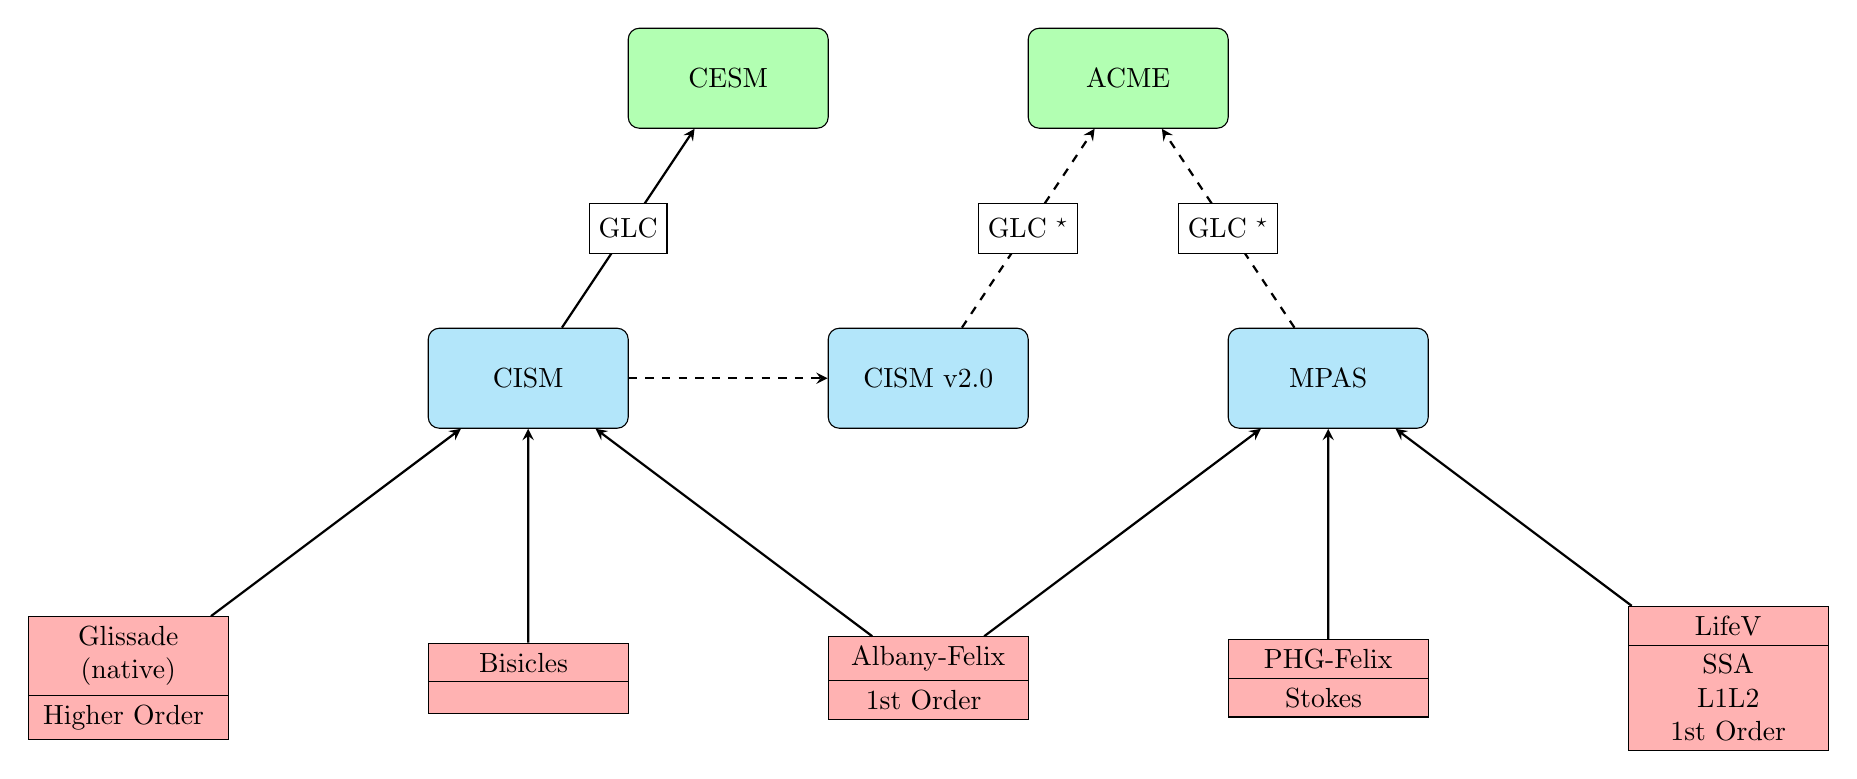
\begin{tikzpicture}{auto}
        \node [climateModel] (CESM) {CESM};
        \node [climateModel] (ACME)   at ([shift={(2in,0)}] CESM) {ACME};
        
        \node [iceModel] (CISM)       at ([shift={(-1in,-1.5in)}] CESM) {CISM};
        \node [iceModel] (CISMv2)   at ([shift={(1in,-1.5in)}] CESM) {CISM v2.0};
        \node [iceModel] (MPAS)       at ([shift={(3in,-1.5in)}] CESM) {MPAS};

        \node [dycore] (Native)       at ([shift={(-4in,-1.5in)}] CISMv2) {
            Glissade \\ (native)
            \nodepart{second} Higher Order
            };
        \node [dycore] (Bisicles)     at ([shift={(-2in,-1.5in)}] CISMv2) {
            Bisicles
            %\nodepart{second} 
            };
        \node [dycore] (Albany-Felix) at ([shift={(0in,-1.5in)}] CISMv2) {
            Albany-Felix
            \nodepart{second} 1st Order
            };
        \node [dycore] (PHG-Felix)    at ([shift={(2in,-1.5in)}] CISMv2) {
            PHG-Felix
            \nodepart{second} Stokes
            };
        \node [dycore] (LifeV)        at ([shift={(4in,-1.5in)}] CISMv2) {
            LifeV
            \nodepart{second} SSA \\ L1L2 \\ 1st Order
            };


        \draw [arrow] (CISM) -- (CESM);
        \draw [dashedArrow] (CISMv2) -- (ACME);
        \draw [dashedArrow] (MPAS) -- (ACME);

        \draw [dashedArrow] (CISM) -- (CISMv2);

        \draw [arrow] (Native) -- (CISM);
        \draw [arrow] (Albany-Felix) -- (CISM);
        \draw [arrow] (Bisicles) -- (CISM);

        \draw [arrow] (Albany-Felix) -- (MPAS);
        \draw [arrow] (PHG-Felix) -- (MPAS);
        \draw [arrow] (LifeV) -- (MPAS);

        \node [textBox] at ([shift={(-.5in,-.75in)}] CESM) {GLC};
        \node [textBox] at ([shift={(1.5in,-.75in)}] CESM) {GLC $^{\star}$};
        \node [textBox] at ([shift={(2.5in,-.75in)}] CESM) {GLC $^{\star}$};

    \end{tikzpicture}

    \vspace{5em}
    $\star \;$ Generalize, split up, ... move glint into the coupler to pass fields
\end{document}
